\documentclass[a4paper,12pt]{article}

% Packages
\usepackage[utf8]{inputenc}
\usepackage{amsmath}
\usepackage{amsfonts}
\usepackage{amssymb}
\usepackage{graphicx}
\usepackage{hyperref}
\usepackage{geometry}
\usepackage{booktabs}
\usepackage{subcaption}
\usepackage{float}
\usepackage{tabularx}

% Page Geometry
\geometry{a4paper, margin=1in}

% Title, Author, and Date
\title{Machine Learning Analysis on AVC and Salary Datasets}
\author{Dragomir Andrei}
\date{\today}

% Document
\begin{document}

\maketitle

\begin{abstract}
This document provides a comprehensive analysis of two machine learning models applied to the given datasets. The analysis includes data preprocessing, model training, evaluation, and comparison of results.
\end{abstract}

\newpage

\tableofcontents
\newpage

\section{Introduction}
In this analysis, we explore the Logistic Regression and the Multy Layer Perceptron models on the AVC and Salary datasets. The goal is to predict the target variable based on the features provided in the datasets.

\section*{Dataset Description}
\section{Medical and Lifestyle Information Dataset}

This dataset contains medical values and relevant lifestyle information for 5110 individuals. The dataset is intended to be used for predicting whether a person is likely to have a cerebrovascular accident (stroke) or not. The target attribute is \textit{cerebrovascular\_accident}, which has binary values indicating the presence (1) or absence (0) of a stroke. The classification task is binary.

The attributes in the dataset are as follows:

\begin{table}[H]
    \centering
    \caption{Attributes of the Medical and Lifestyle Information Dataset}
    \begin{tabular}{|l|l|p{10cm}|}
    \hline
    \textbf{Attribute} & \textbf{Type} & \textbf{Description} \\ \hline
    mean\_blood\_sugar\_level & numeric & The average blood sugar level over the observation period. \\ \hline
    cardiovascular\_issues & categorical & Indicates if the subject has a history of cardiovascular issues. Possible values: 0, 1. \\ \hline
    job\_category & categorical & The domain in which the person works. Possible values: child, entrepreneurial, N\_work\_history, private\_sector, public\_sector. \\ \hline
    body\_mass\_indicator & numeric & The body mass index indicating if the person is underweight, normal weight, overweight, or obese. \\ \hline
    sex & categorical & The gender of the person. Possible values: F, M. \\ \hline
    tobacco\_usage & categorical & Indicator for tobacco use, present or past. Possible values: ex-smoker, smoker, non-smoker. \\ \hline
    high\_blood\_pressure & categorical & Binary attribute indicating if a person suffers from high blood pressure. Possible values: 0, 1. \\ \hline
    married & categorical & Binary attribute indicating if the person has ever been married. Possible values: Y, N. \\ \hline
    living\_area & categorical & Type of area where the person has lived most of their life. Possible values: City, Countryside. \\ \hline
    years\_old & numeric & The age of the person in years. \\ \hline
    chaotic\_sleep & categorical & Binary attribute for an irregular sleep schedule. Possible values: 0, 1. \\ \hline
    analysis\_results & numeric & Results of the person's medical tests, which may include various measurements and health indicators. \\ \hline
    biological\_age\_index & numeric & An index estimating the biological age of a person based on various factors such as lifestyle and health status. \\ \hline
    cerebrovascular\_accident & categorical & Binary indicator of whether the person has had a stroke. Possible values: 0, 1. \\ \hline
    \end{tabular}
    \end{table}
    
\section{Employee Information Dataset}

This dataset contains personal, educational, and professional information of various employees. The objective of this dataset is the binary classification of employees into categories of earning above or below \$50K per year. The classification task is binary.

The attributes in the dataset are as follows:
\begin{table}[H]
\centering
\caption{Attributes of the Employee Information Dataset}
\begin{tabular}{|l|l|p{10cm}|}
\hline
\textbf{Attribute} & \textbf{Type} & \textbf{Description} \\ \hline
fnl & numeric & Socio-economic characteristic of the population from which the individual comes. \\ \hline
hpw & numeric & Number of hours worked per week. \\ \hline
relation & categorical & The type of relationship in which the individual is involved. \\ \hline
gain & numeric & Capital gain. \\ \hline
country & categorical & Country of origin. \\ \hline
job & categorical & The individual's occupation. \\ \hline
edu\_int & numeric & Number of years of education. \\ \hline
years & numeric & Age of the individual. \\ \hline
loss & numeric & Capital loss. \\ \hline
work\_type & categorical & Type of occupation. \\ \hline
partner & categorical & Type of partner the individual has. \\ \hline
edu & categorical & Type of education of the individual. \\ \hline
gender & categorical & Gender of the individual. \\ \hline
race & categorical & Race of the individual. \\ \hline
prod & numeric & Capital production. \\ \hline
gtype & categorical & Type of work contract. \\ \hline
\end{tabular}
\end{table}
    
\section{Attribute Type Identification}

Before utilizing a machine learning model for a dataset, it is crucial to identify the types of features in the dataset and their values. Understanding the nature of the attributes helps in selecting appropriate preprocessing techniques and models. The key distinctions among the types of attributes in the provided datasets are as follows:

\subsection{Continuous Numerical Attributes}

Continuous numerical attributes are features that can take any value within a given range. These attributes are measured on a continuous scale and can be divided into finer increments. Examples from the datasets include:

\begin{itemize}
    \item \textbf{mean\_blood\_sugar\_level}: Average blood sugar level measured over the observation period.
    \item \textbf{body\_mass\_indicator}: Body mass index indicating whether a person is underweight, normal weight, overweight, or obese.
    \item \textbf{years\_old}: Age of the person in years.
    \item \textbf{analysis\_results}: Results of medical tests.
    \item \textbf{biological\_age\_index}: An index estimating the biological age of a person based on various factors.
    \item \textbf{fnl}: Socio-economic characteristic of the population the individual comes from.
    \item \textbf{hpw}: Number of hours worked per week.
    \item \textbf{gain}: Capital gain.
    \item \textbf{edu\_int}: Number of years of education.
    \item \textbf{years}: Age of the individual.
    \item \textbf{loss}: Capital loss.
    \item \textbf{prod}: Capital production.
\end{itemize}

\subsection{Discrete Attributes}

Discrete attributes are features that take on a finite number of distinct values. These values are often categorical and can be counted in whole numbers. Examples from the datasets include:

\begin{itemize}
    \item \textbf{cardiovascular\_issues}: Whether the subject has a history of cardiovascular issues (0 or 1).
    \item \textbf{sex}: Gender of the person (F or M).
    \item \textbf{tobacco\_usage}: Indicator for smokers, either past or present (ex-smoker, smoker, non-smoker).
    \item \textbf{high\_blood\_pressure}: Indicator if a person has high blood pressure (0 or 1).
    \item \textbf{married}: Whether the person has ever been married (Y or N).
    \item \textbf{living\_area}: Type of area where the person has lived most of their life (City or Countryside).
    \item \textbf{chaotic\_sleep}: Indicator for an irregular sleep schedule (0 or 1).
    \item \textbf{cerebrovascular\_accident}: Indicator if the person has had a stroke (0 or 1).
    \item \textbf{relation}: Type of relationship the individual is involved in.
    \item \textbf{country}: Country of origin.
    \item \textbf{job}: Job of the individual.
    \item \textbf{work\_type}: Type of job.
    \item \textbf{partner}: Type of partner the individual has.
    \item \textbf{edu}: Type of education of the individual.
    \item \textbf{gender}: Gender of the individual.
    \item \textbf{race}: Race of the individual.
    \item \textbf{gtype}: Type of work contract.
    \item \textbf{job\_category}: Domain in which the person works.
\end{itemize}


Recognizing these distinctions helps in choosing the right methods for handling the data during preprocessing. For instance, continuous numerical attributes might require normalization or standardization, discrete attributes might need encoding, and ordinal attributes might need ordinal encoding to maintain the order information. Properly identifying and classifying the attributes ensures that the machine learning models can effectively learn from the data and make accurate predictions.

\section{Numeric Attributes Analysis}

In this section, we analyze the numeric attributes of the two datasets provided. The analysis includes the number of non-missing values, mean value, standard deviation, minimum value, 25th percentile, 50th percentile (median), 75th percentile, and maximum value for each numeric attribute.

\subsection{Healthcare Dataset}

\begin{table}[h!]
\centering
\caption{Statistics of Numeric Attributes in the Healthcare Dataset}
\vspace{0.5cm}
\small
\begin{tabularx}{\textwidth}{|l|X|X|X|X|X|X|X|X|}
\hline
\textbf{Attribute} & \textbf{No-miss} & \textbf{Mean} & \textbf{Std Dev} & \textbf{Min} & \textbf{25th Pctl} & \textbf{Mid} & \textbf{75th Pctl} & \textbf{Max} \\
\hline
mean\_blood\_sugar\_level & 5110 & 106.15 & 45.28 & 55.12 & 77.25 & 91.89 & 114.09 & 271.74 \\
body\_mass\_indicator & 4909 & 28.89 & 7.85 & 10.30 & 23.50 & 28.10 & 33.10 & 97.60 \\
years\_old & 5110 & 46.57 & 26.59 & 0.08 & 26.00 & 47.00 & 63.75 & 134.00 \\
analysis\_results & 4599 & 323.52 & 101.58 & 104.83 & 254.65 & 301.03 & 362.82 & 756.81 \\
biological\_age\_index & 5110 & 134.78 & 50.40 & -15.11 & 96.71 & 136.37 & 172.51 & 266.99 \\
\hline
\end{tabularx}
\normalsize
\end{table}

\textbf{Comments:}
\begin{itemize}
    \item The \textbf{mean\_blood\_sugar\_level} has a mean of 106.15 with a standard deviation of 45.28, indicating a wide range of values.
    \item The \textbf{body\_mass\_indicator} shows a mean of 28.89, suggesting that on average, individuals fall into the overweight category.
    \item The \textbf{years\_old} attribute ranges from 0.08 to 134 years, with a median of 47 years.
    \item The \textbf{analysis\_results} attribute has significant variability, as indicated by its standard deviation of 101.58.
    \item The \textbf{biological\_age\_index} has negative values, which may need to be investigated further for data correctness.
\end{itemize}

\subsection{Employee Dataset}

\begin{table}[h!]
\centering
\caption{Statistics of Numeric Attributes in the Employee Dataset}
\vspace{0.5cm}
\small
\begin{tabularx}{\textwidth}{|l|X|X|X|X|X|X|X|X|}
\hline
\textbf{Attribute} & \textbf{No-miss} & \textbf{Mean} & \textbf{Std Dev} & \textbf{Min} & \textbf{25th Pctl} & \textbf{Mid} & \textbf{75th Pctl} & \textbf{Max} \\
\hline
fnl & 9999 & 190352.9 & 106070.8 & 19214 & 118282.5 & 178472 & 237311 & 1455435 \\
hpw & 9199 & 40.42 & 12.52 & 1.0 & 40.0 & 40.0 & 45.0 & 99.0 \\
gain & 9999 & 979.85 & 7003.80 & 0.0 & 0.0 & 0.0 & 0.0 & 99999.0 \\
edu\_int & 9999 & 14.26 & 24.77 & 1.0 & 9.0 & 10.0 & 13.0 & 206.0 \\
years & 9999 & 38.65 & 13.75 & 17.0 & 28.0 & 37.0 & 48.0 & 90.0 \\
loss & 9999 & 84.11 & 394.04 & 0.0 & 0.0 & 0.0 & 0.0 & 3770.0 \\
prod & 9999 & 2014.93 & 14007.60 & -28.0 & 42.0 & 57.0 & 77.0 & 200125.0 \\
\hline
\end{tabularx}
\normalsize
\end{table}

\textbf{Comments:}
\begin{itemize}
    \item The \textbf{fnl} attribute has a high mean value and a wide range, indicating significant differences in the socio-economic status of individuals.
    \item The \textbf{hpw} (hours per week) attribute shows that most individuals work around 40 hours per week.
    \item The \textbf{gain} and \textbf{loss} attributes have a high standard deviation, indicating that only a few individuals have large capital gains or losses.
    \item The \textbf{edu\_int} (years of education) attribute shows that the majority of individuals have around 10 to 13 years of education.
    \item The \textbf{years} attribute shows an average age of around 38.65 years, with a minimum of 17 and a maximum of 90 years.
    \item The \textbf{prod} attribute has a high standard deviation, indicating variability in capital production.
\end{itemize}

\newpage

\section{Numeric Ranges for Attributes}

In this section, we present the boxplots for the numeric attributes in the datasets to visualize the distribution and identify any potential outliers.

\subsection{Healthcare Dataset}

\begin{figure}[h!]
    \centering
    \begin{subfigure}[b]{0.45\textwidth}
        \centering
        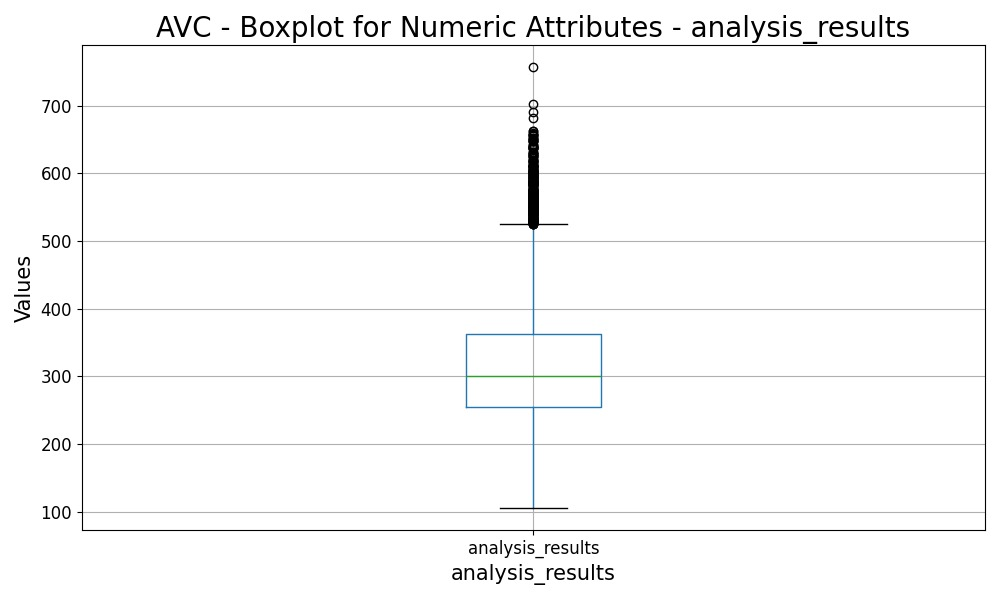
\includegraphics[width=\textwidth]{Resources/Boxplot_analysis_results.jpeg}
        \caption{Analysis Results}
        \label{fig:analysis_results}
    \end{subfigure}
    \hfill
    \begin{subfigure}[b]{0.45\textwidth}
        \centering
        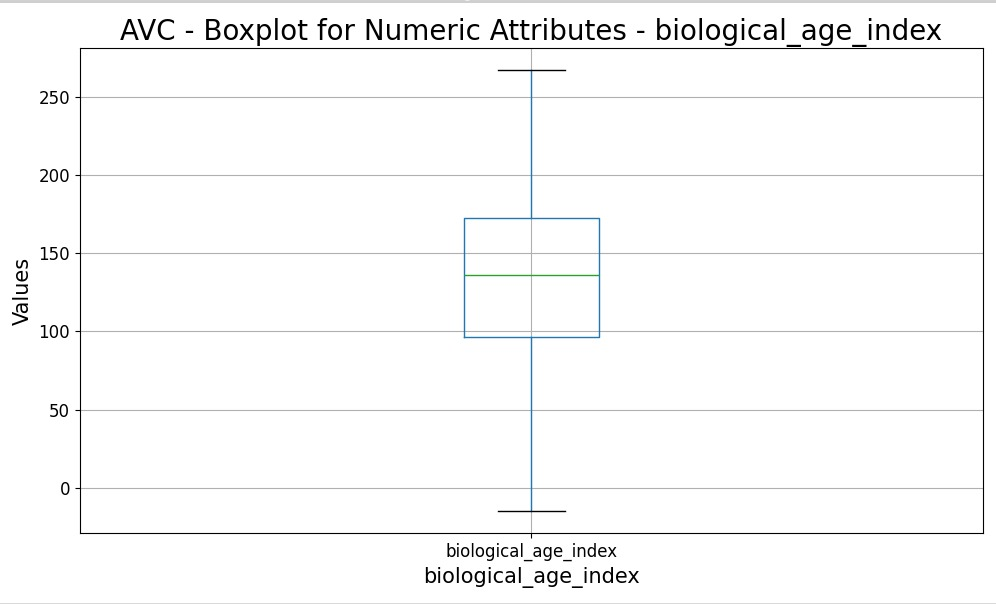
\includegraphics[width=\textwidth]{Resources/Boxplot_biological_index.jpeg}
        \caption{Biological Age Index}
        \label{fig:biological_index}
    \end{subfigure}
    
    \vspace{0.5cm}
    
    \begin{subfigure}[b]{0.45\textwidth}
        \centering
        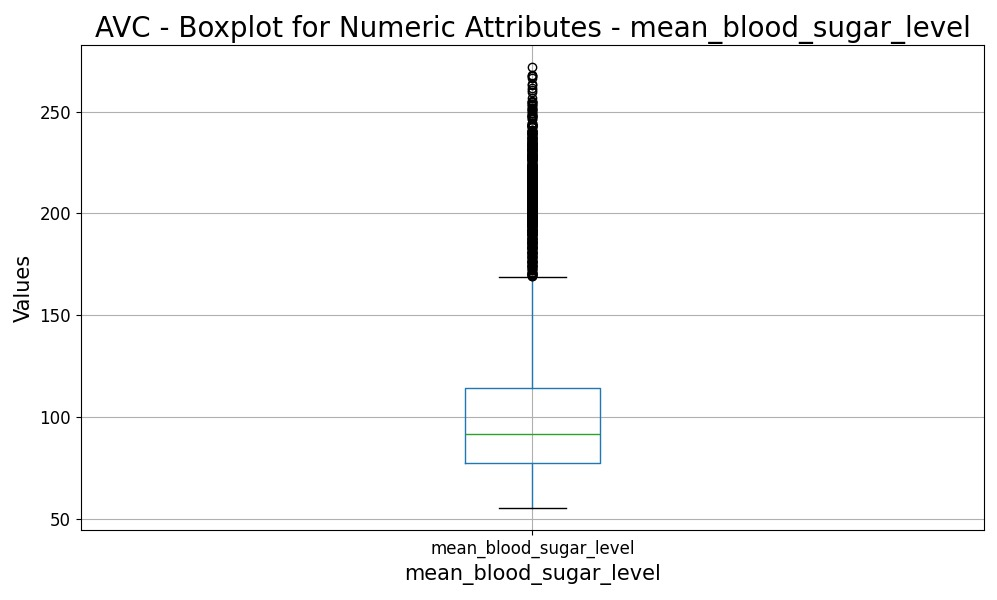
\includegraphics[width=\textwidth]{Resources/Boxplot_blood_sugar_level.jpeg}
        \caption{Mean Blood Sugar Level}
        \label{fig:blood_sugar_level}
    \end{subfigure}
    \hfill
    \begin{subfigure}[b]{0.45\textwidth}
        \centering
        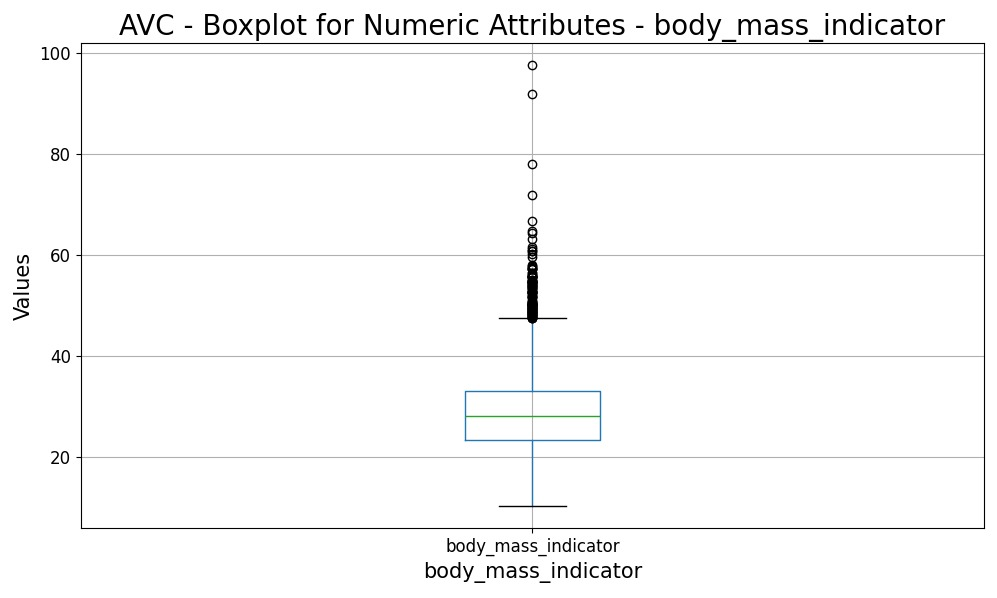
\includegraphics[width=\textwidth]{Resources/Boxplot_body_mass_indicator.jpeg}
        \caption{Body Mass Indicator}
        \label{fig:body_mass_indicator}
    \end{subfigure}
    
    \vspace{0.5cm}
    
    \begin{subfigure}[b]{0.45\textwidth}
        \centering
        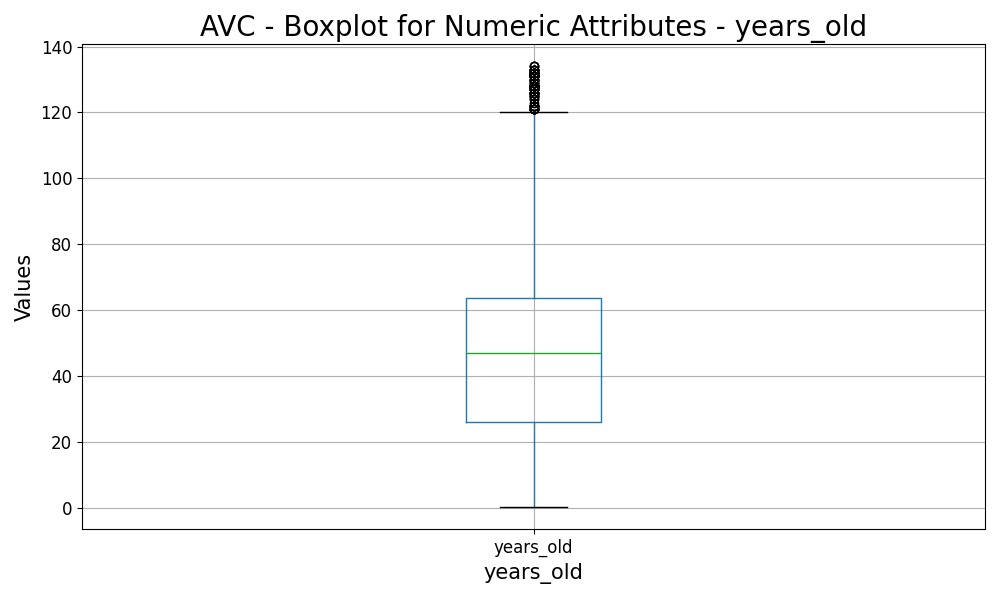
\includegraphics[width=\textwidth]{Resources/Boxplot_years_old.jpeg}
        \caption{Years Old}
        \label{fig:years_old}
    \end{subfigure}
    
    \caption{Boxplots for Healthcare Dataset Numeric Attributes}
\end{figure}

\newpage
\subsection{Employee Dataset}

\begin{figure}[h!]
    \centering
    \begin{subfigure}[b]{0.45\textwidth}
        \centering
        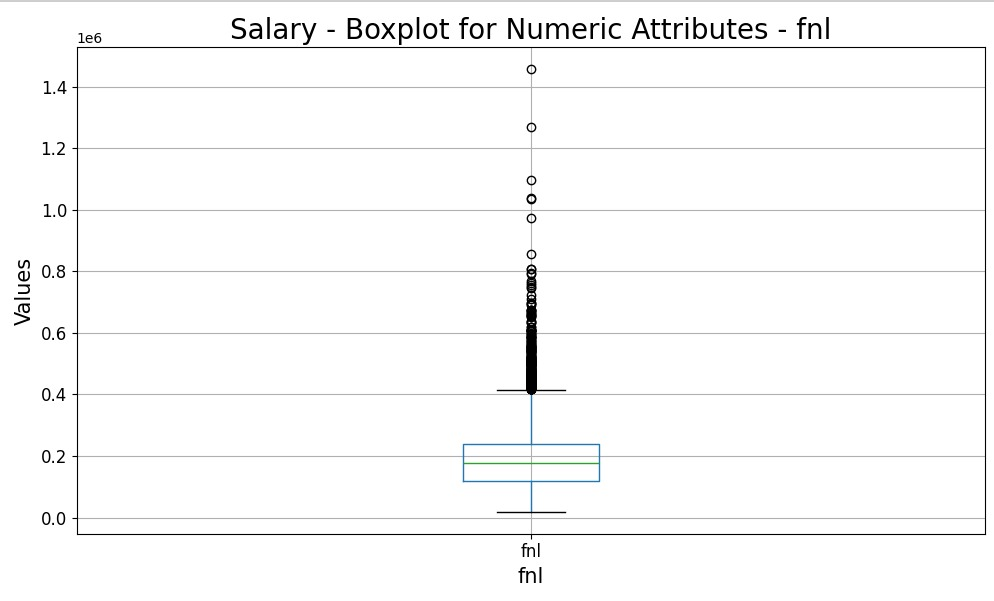
\includegraphics[width=\textwidth]{Resources/Boxplot_fnl.jpeg}
        \caption{FNL}
        \label{fig:fnl}
    \end{subfigure}
    \hfill
    \begin{subfigure}[b]{0.45\textwidth}
        \centering
        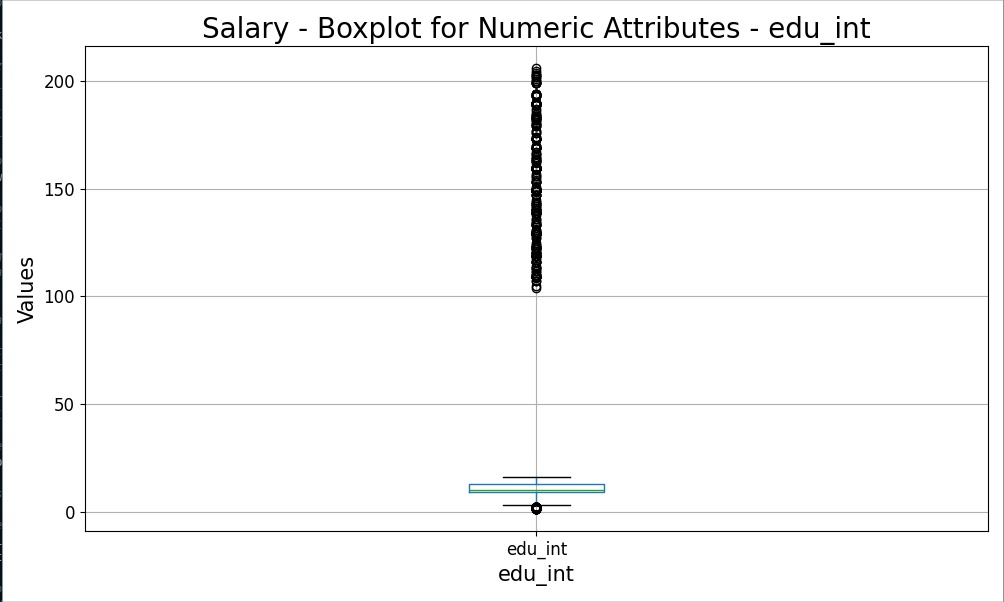
\includegraphics[width=\textwidth]{Resources/Boxplot_edu_int.jpeg}
        \caption{Education (Years)}
        \label{fig:edu_int}
    \end{subfigure}
    
    \vspace{0.5cm}
    
    \begin{subfigure}[b]{0.45\textwidth}
        \centering
        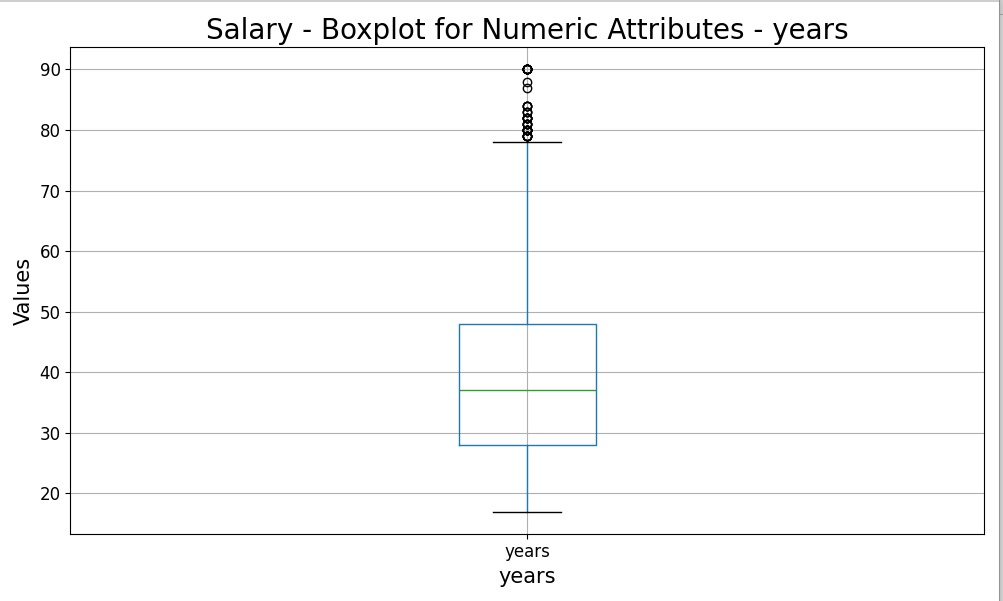
\includegraphics[width=\textwidth]{Resources/Boxplot_years.jpeg}
        \caption{Years}
        \label{fig:years}
    \end{subfigure}
    \hfill
    \begin{subfigure}[b]{0.45\textwidth}
        \centering
        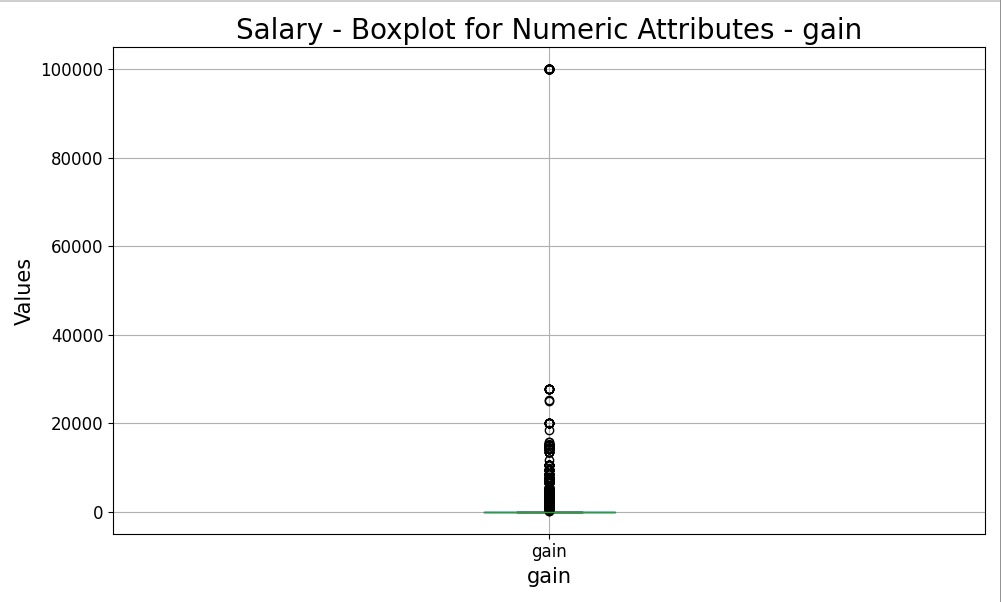
\includegraphics[width=\textwidth]{Resources/Boxplot_gain.jpeg}
        \caption{Gain}
        \label{fig:gain}
    \end{subfigure}
    
    \vspace{0.5cm}
    
    \begin{subfigure}[b]{0.45\textwidth}
        \centering
        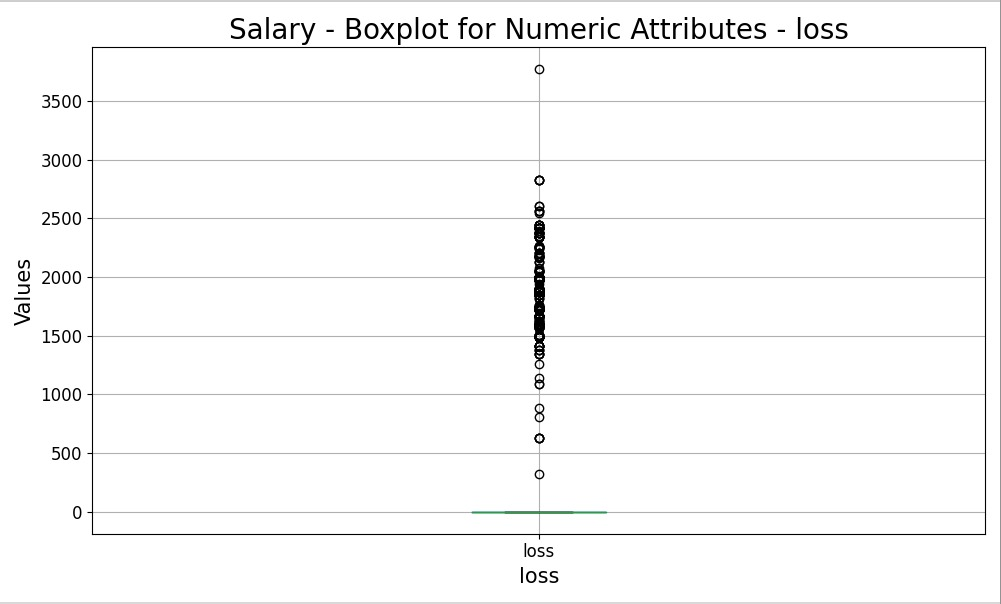
\includegraphics[width=\textwidth]{Resources/Boxplot_loss.jpeg}
        \caption{Loss}
        \label{fig:loss}
    \end{subfigure}
    \hfill
    \begin{subfigure}[b]{0.45\textwidth}
        \centering
        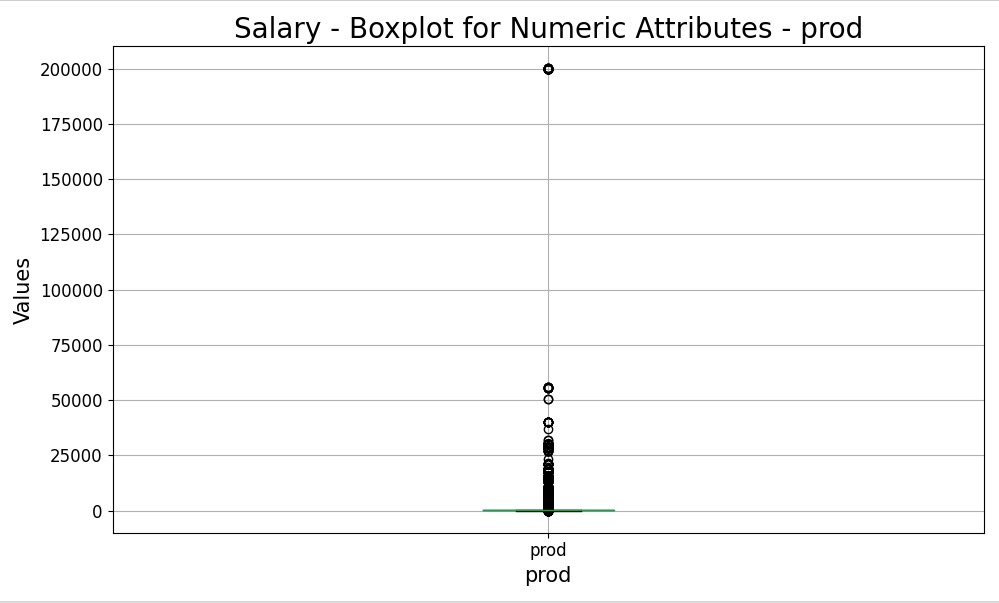
\includegraphics[width=\textwidth]{Resources/Boxplot_prod.jpeg}
        \caption{Prod}
        \label{fig:prod}
    \end{subfigure}
    
    \caption{Boxplots for Employee Dataset Numeric Attributes}
\end{figure}

\newpage

\section{Categorical Attributes Analysis}

In this section, we analyze the categorical attributes of the datasets. The tables below present the attributes along with the number of non-missing values and the number of unique values for each attribute.

\subsection{Healthcare Dataset}

\begin{table}[h!]
\centering
\caption{Categorical Attributes - Healthcare Dataset}
\vspace{0.5cm}
\small
\begin{tabularx}{\textwidth}{|l|X|X|}
\hline
\textbf{Attribute} & \textbf{Number of Non-Missing Values} & \textbf{Number of Unique Values} \\ \hline
cardiovascular\_issues & 5110 & 2 \\ \hline
job\_category & 5110 & 5 \\ \hline
sex & 5110 & 2 \\ \hline
tobacco\_usage & 5110 & 4 \\ \hline
high\_blood\_pressure & 5110 & 2 \\ \hline
married & 4599 & 2 \\ \hline
living\_area & 5110 & 2 \\ \hline
chaotic\_sleep & 5110 & 2 \\ \hline
cerebrovascular\_accident & 5110 & 2 \\ \hline
\end{tabularx}
\normalsize
\end{table}

\subsection{Employee Dataset}

\begin{table}[h!]
\centering
\caption{Categorical Attributes - Employee Dataset}
\vspace{0.5cm}
\small
\begin{tabularx}{\textwidth}{|l|X|X|}
\hline
\textbf{Attribute} & \textbf{Number of Non-Missing Values} & \textbf{Number of Unique Values} \\ \hline
relation & 9999 & 6 \\ \hline
country & 9999 & 41 \\ \hline
job & 9999 & 14 \\ \hline
work\_type & 9999 & 9 \\ \hline
partner & 9999 & 7 \\ \hline
edu & 9999 & 16 \\ \hline
gender & 9199 & 2 \\ \hline
race & 9999 & 5 \\ \hline
gtype & 9999 & 2 \\ \hline
money & 9999 & 2 \\ \hline
\end{tabularx}
\normalsize
\end{table}

\newpage
\subsection{Comments}

The healthcare dataset includes several categorical attributes such as `cardiovascular\_issues`, `job\_category`, `sex`, and `tobacco\_usage`. Each of these attributes has a varying number of unique values, indicating different levels of categorization. For instance, `tobacco\_usage` has four unique values, while `sex` has only two. It is also noted that the `married` attribute has fewer non-missing values compared to others, which might require special handling during data preprocessing.

The employee dataset, on the other hand, contains a wider range of categorical attributes with a larger variety of unique values, especially for `country` and `edu`, which have 41 and 16 unique values, respectively. Attributes like `gender` and `gtype` are binary, which simplifies their processing. The variety in the number of unique values across different attributes in both datasets indicates the complexity and diversity of the data, which must be carefully considered during the feature engineering and model building stages.

\section{Categorical Distribution for Attributes}

\subsection{Healthcare Dataset}
\begin{figure}[H]
    \centering
    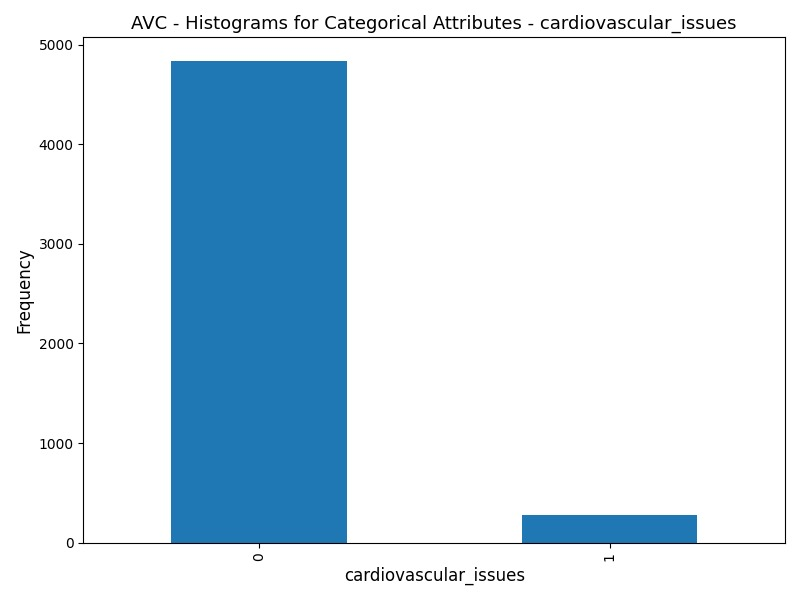
\includegraphics[width=0.8\textwidth]{Resources/histogram_cardio_issues.jpeg}
    \caption{Cardiovascular Issues}
\end{figure}

\begin{figure}[H]
    \centering
    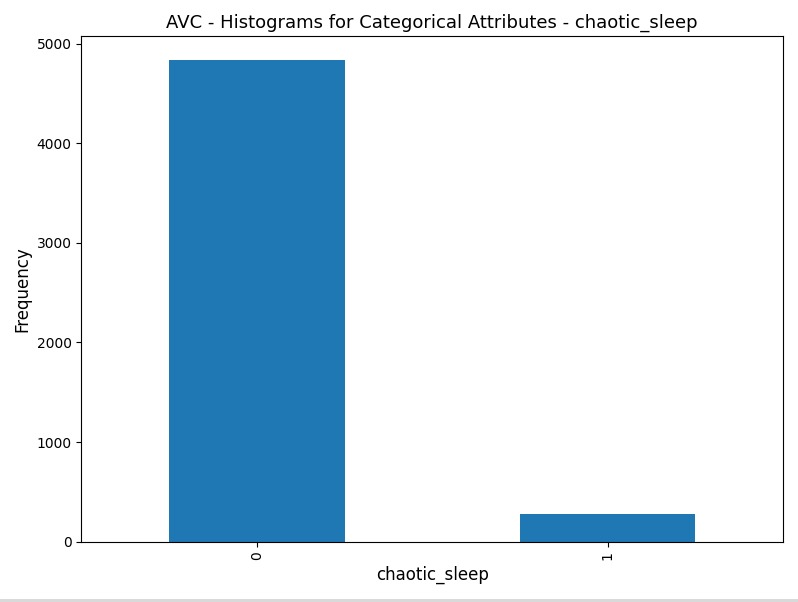
\includegraphics[width=0.8\textwidth]{Resources/histogram_chaotic_sleep.jpeg}
    \caption{Chaotic Sleep}
\end{figure}

\begin{figure}[H]
    \centering
    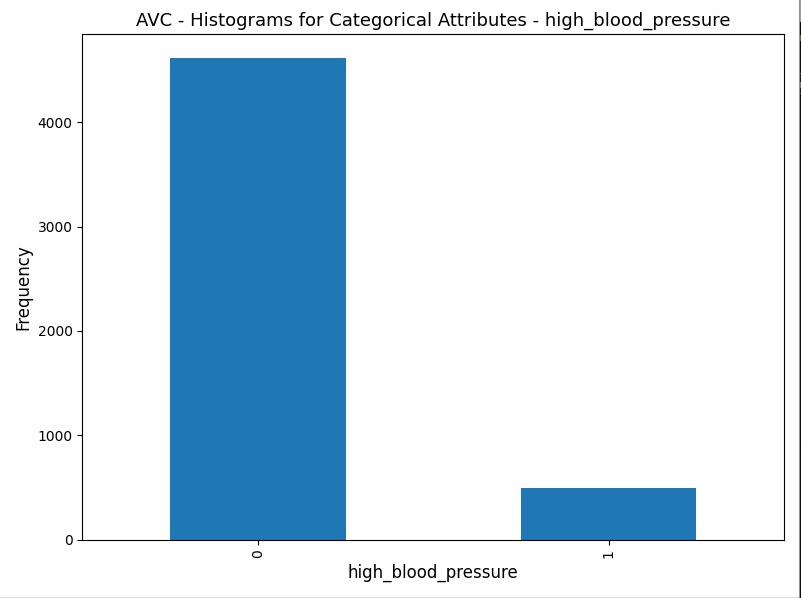
\includegraphics[width=0.8\textwidth]{Resources/histogram_high_blood_pressure.jpeg}
    \caption{High Blood Pressure}
\end{figure}

\begin{figure}[H]
    \centering
    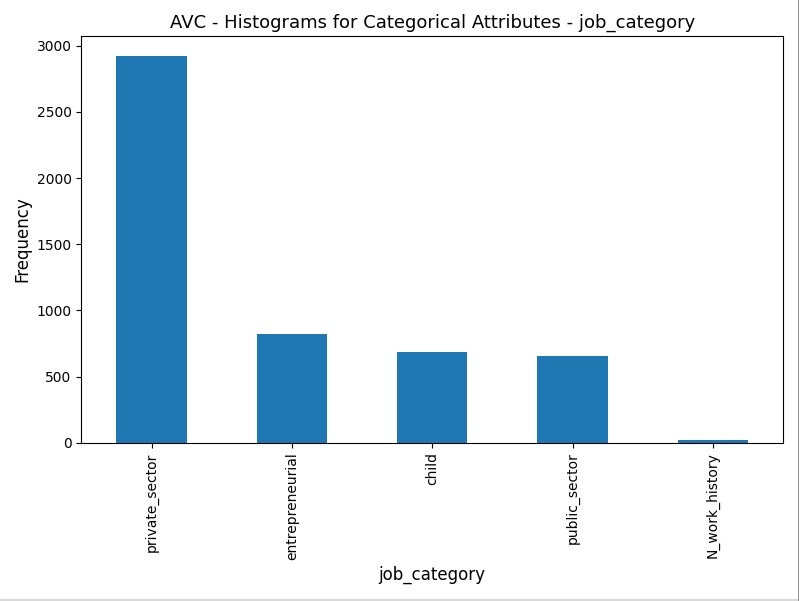
\includegraphics[width=0.8\textwidth]{Resources/histogram_job_cat.jpeg}
    \caption{Job Category}
\end{figure}

\begin{figure}[H]
    \centering
    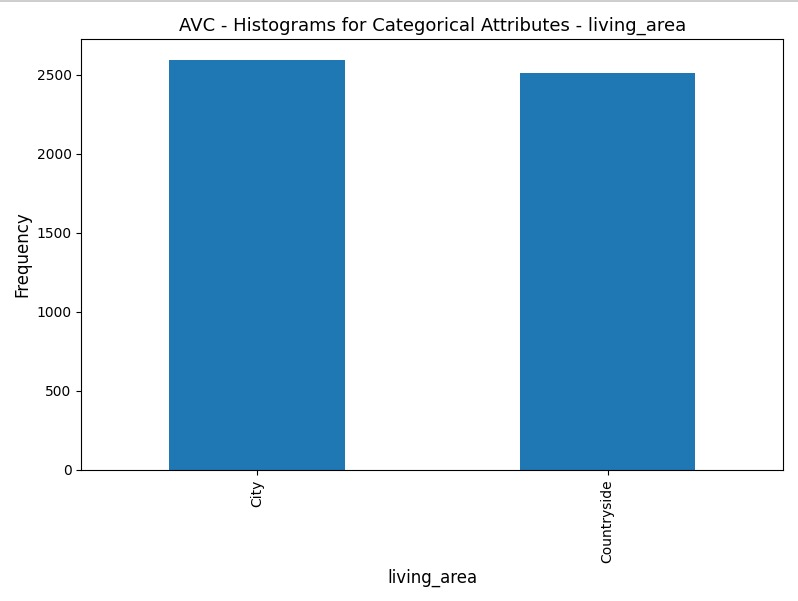
\includegraphics[width=0.8\textwidth]{Resources/histogram_living_area.jpeg}
    \caption{Living Area}
\end{figure}

\begin{figure}[H]
    \centering
    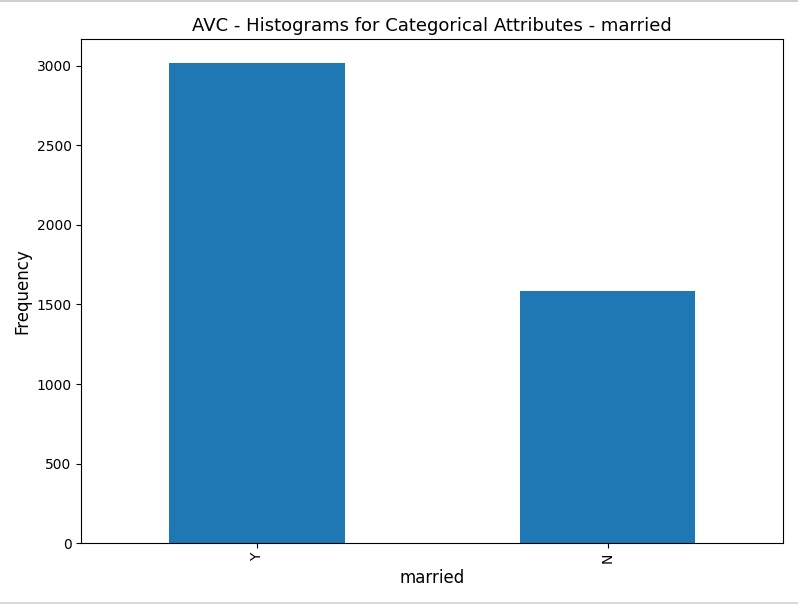
\includegraphics[width=0.8\textwidth]{Resources/histogram_married.jpeg}
    \caption{Married}
\end{figure}

\begin{figure}[H]
    \centering
    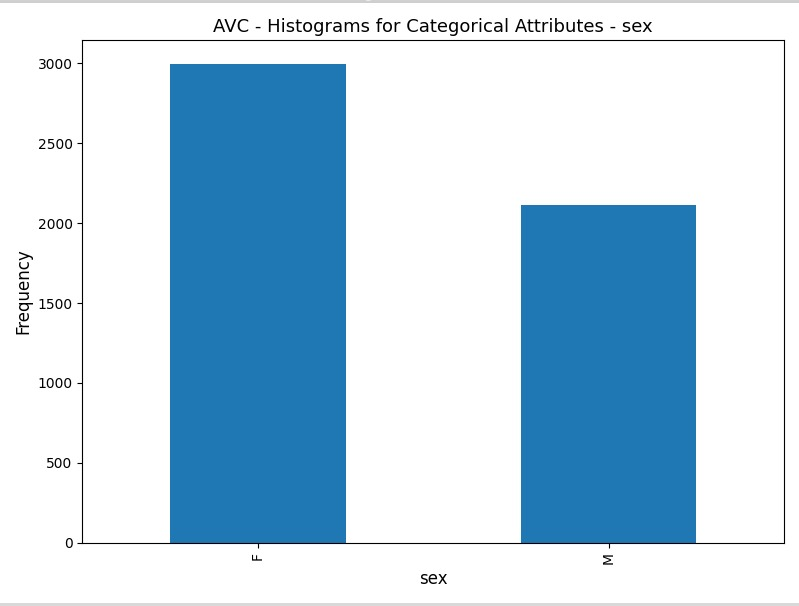
\includegraphics[width=0.8\textwidth]{Resources/histogram_sex.jpeg}
    \caption{Sex}
\end{figure}

\begin{figure}[H]
    \centering
    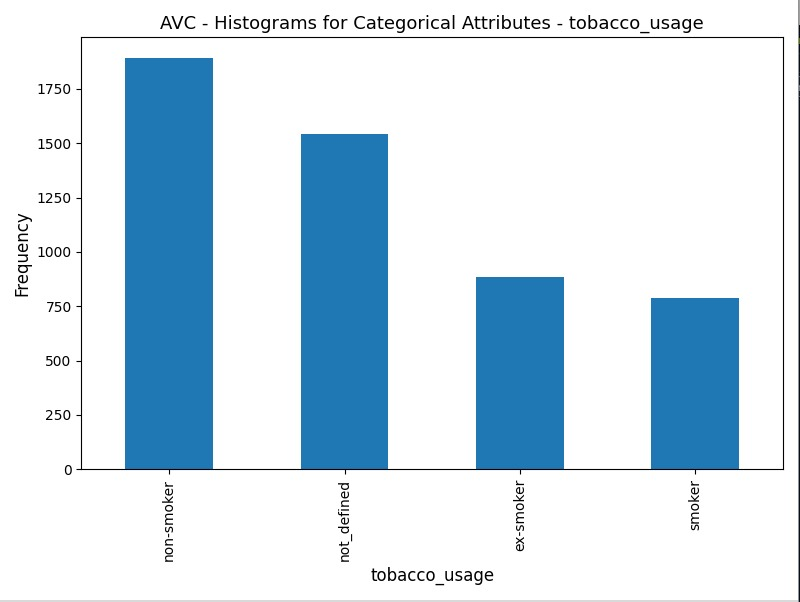
\includegraphics[width=0.8\textwidth]{Resources/histogram_tobacco_usage.jpeg}
    \caption{Tobacco Usage}
\end{figure}

\subsection{Salary Dataset}
\begin{figure}[H]
    \centering
    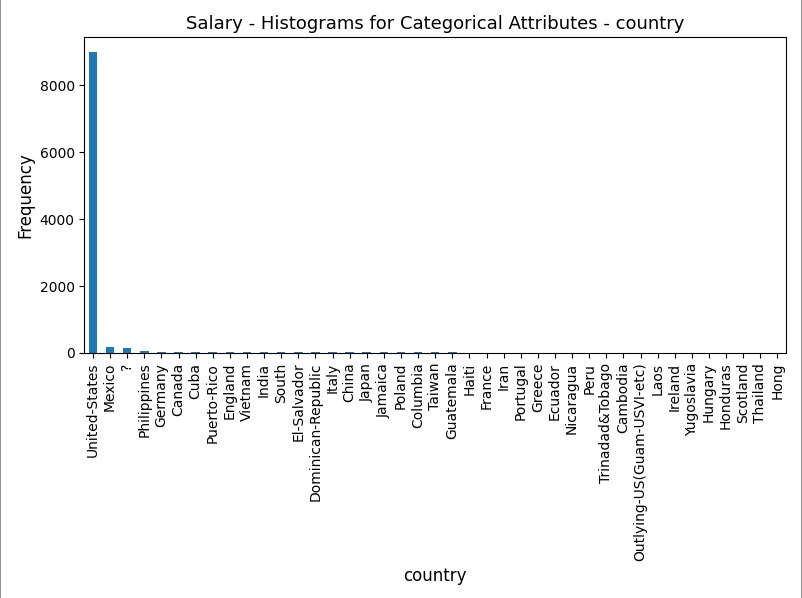
\includegraphics[width=0.8\textwidth]{Resources/histogram_country.jpeg}
    \caption{Country}
\end{figure}

\begin{figure}[H]
    \centering
    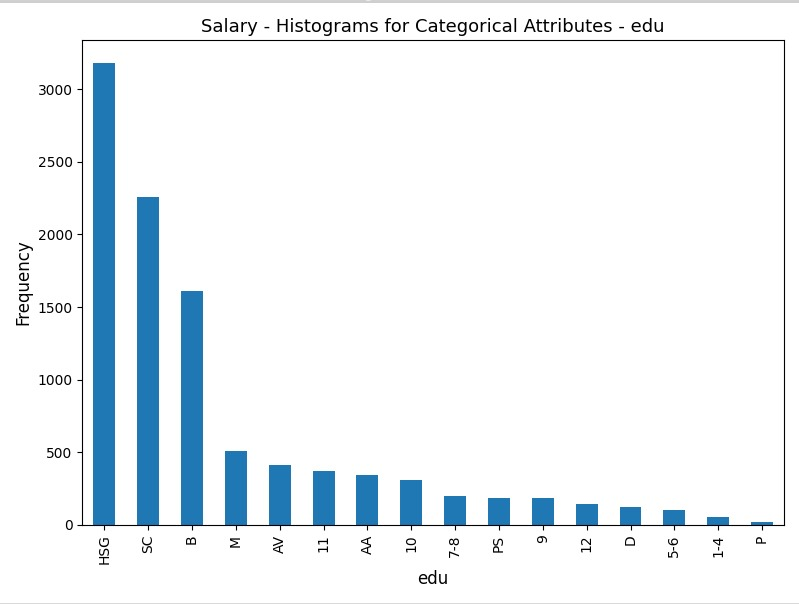
\includegraphics[width=0.8\textwidth]{Resources/histogram_edu.jpeg}
    \caption{Education}
\end{figure}

\begin{figure}[H]
    \centering
    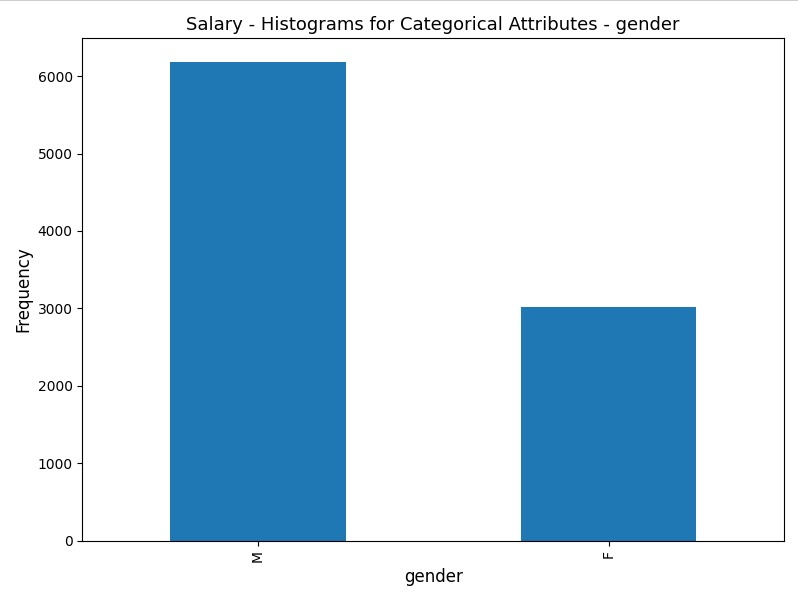
\includegraphics[width=0.8\textwidth]{Resources/histogram_gender.jpeg}
    \caption{Gender}
\end{figure}

\begin{figure}[H]
    \centering
    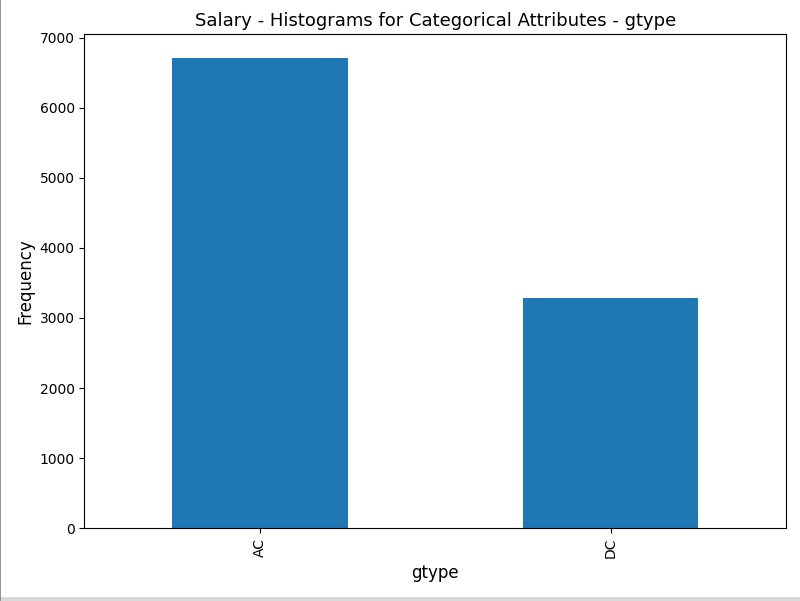
\includegraphics[width=0.8\textwidth]{Resources/histogram_gtype.jpeg}
    \caption{Job Type}
\end{figure}

\begin{figure}[H]
    \centering
    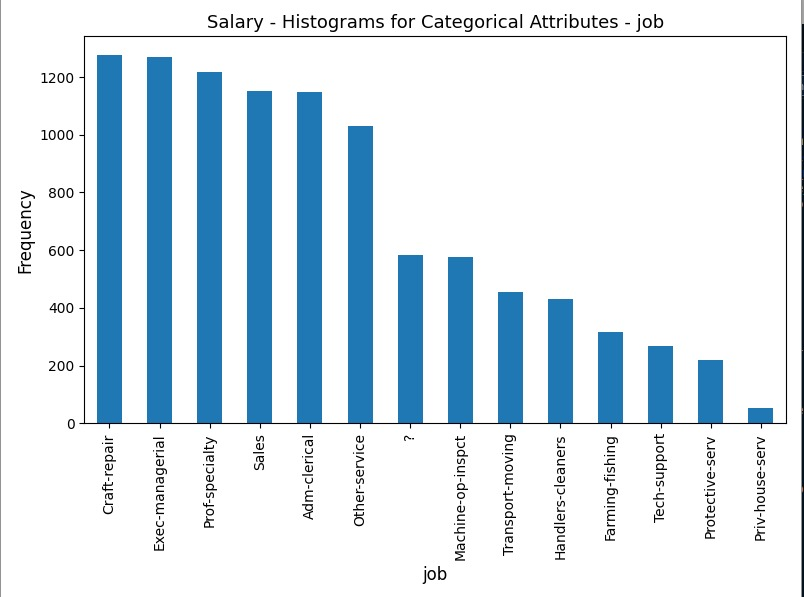
\includegraphics[width=0.8\textwidth]{Resources/histogram_job.jpeg}
    \caption{Job}
\end{figure}

\begin{figure}[H]
    \centering
    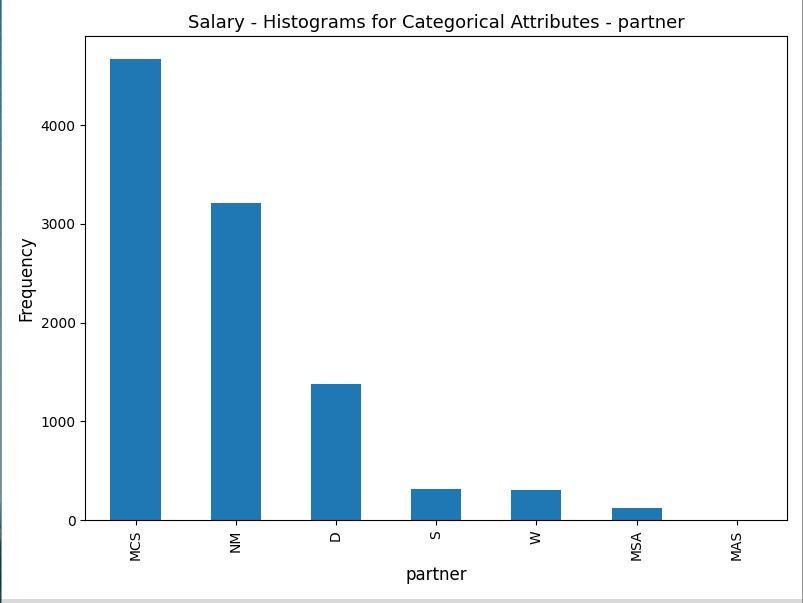
\includegraphics[width=0.8\textwidth]{Resources/histogram_partner.jpeg}
    \caption{Partner}
\end{figure}

\begin{figure}[H]
    \centering
    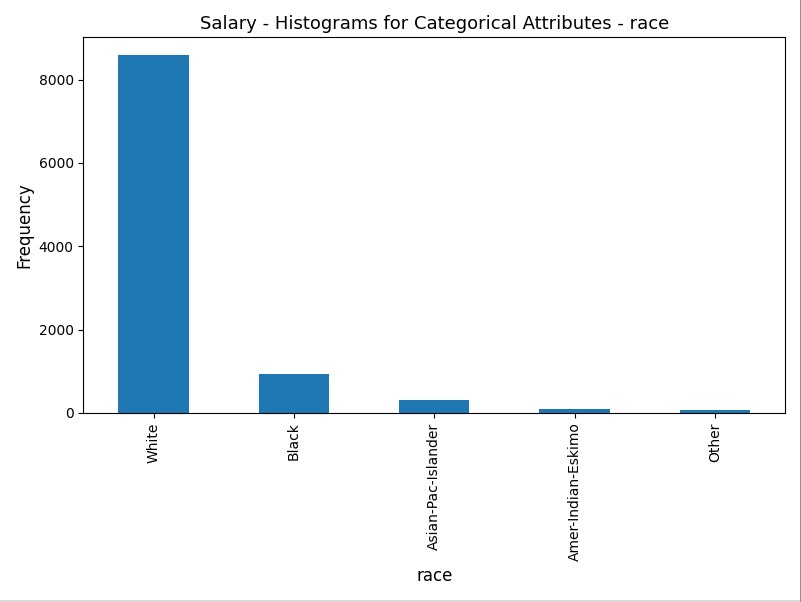
\includegraphics[width=0.8\textwidth]{Resources/histogram_race.jpeg}
    \caption{Race}
\end{figure}

\begin{figure}[H]
    \centering
    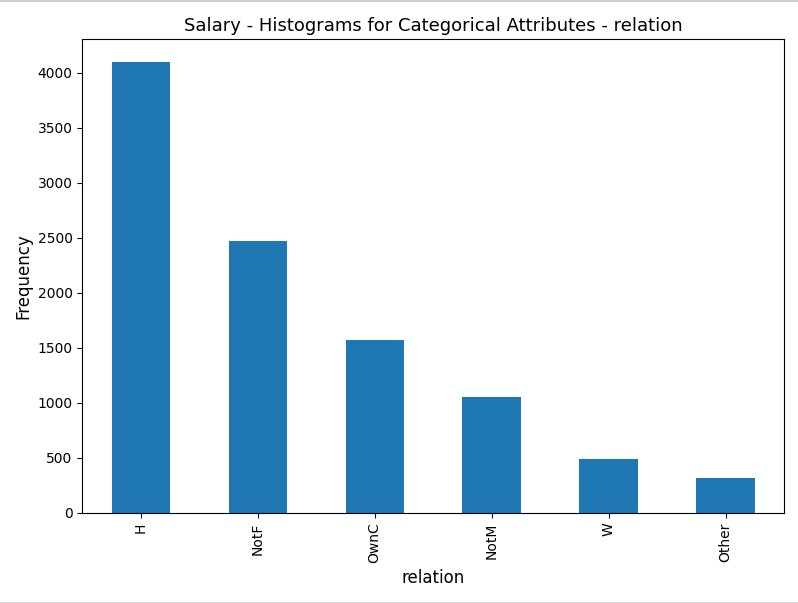
\includegraphics[width=0.8\textwidth]{Resources/histogram_relation.jpeg}
    \caption{Relation}
\end{figure}

\begin{figure}[H]
    \centering
    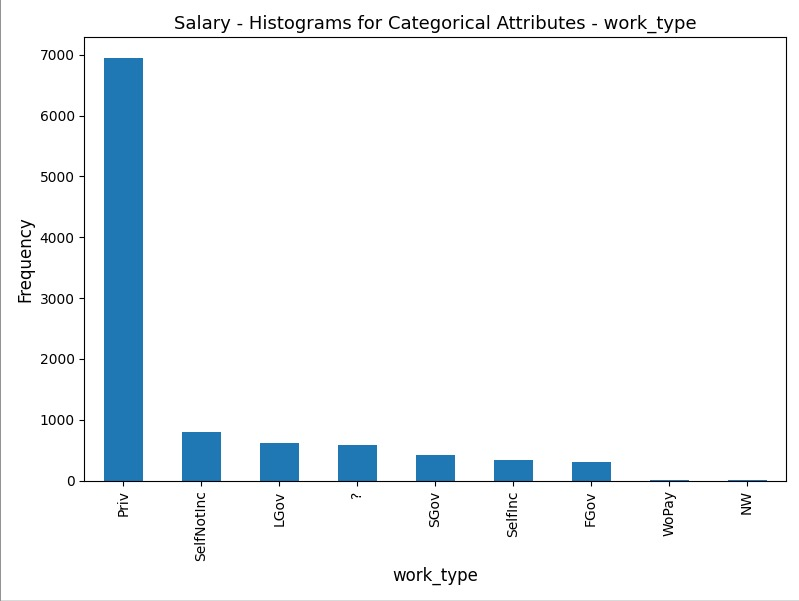
\includegraphics[width=0.8\textwidth]{Resources/histogram_work_type.jpeg}
    \caption{Work Type}
\end{figure}

\newpage

\section{Class Balance}
This section presents the class balance for both the AVC and Salary datasets. The class balance is an important aspect to consider as it influences the evaluation metrics we should focus on.

\subsection{AVC Dataset}
\begin{figure}[h!]
    \centering
    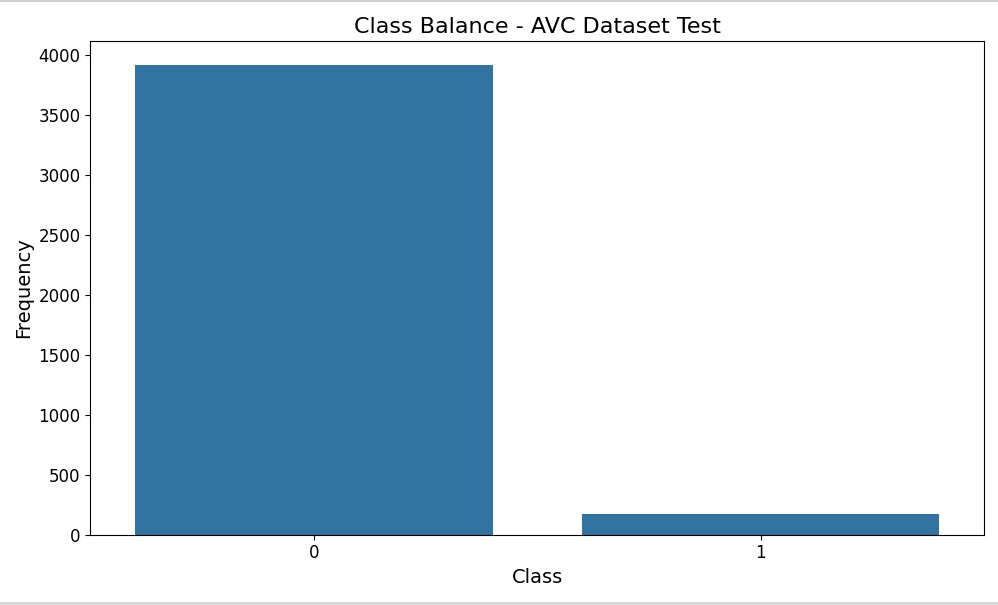
\includegraphics[width=0.8\textwidth]{Resources/class_balance_avc_test.jpeg}
    \caption{Class Balance - AVC Dataset Test}
\end{figure}

\begin{figure}[h!]
    \centering
    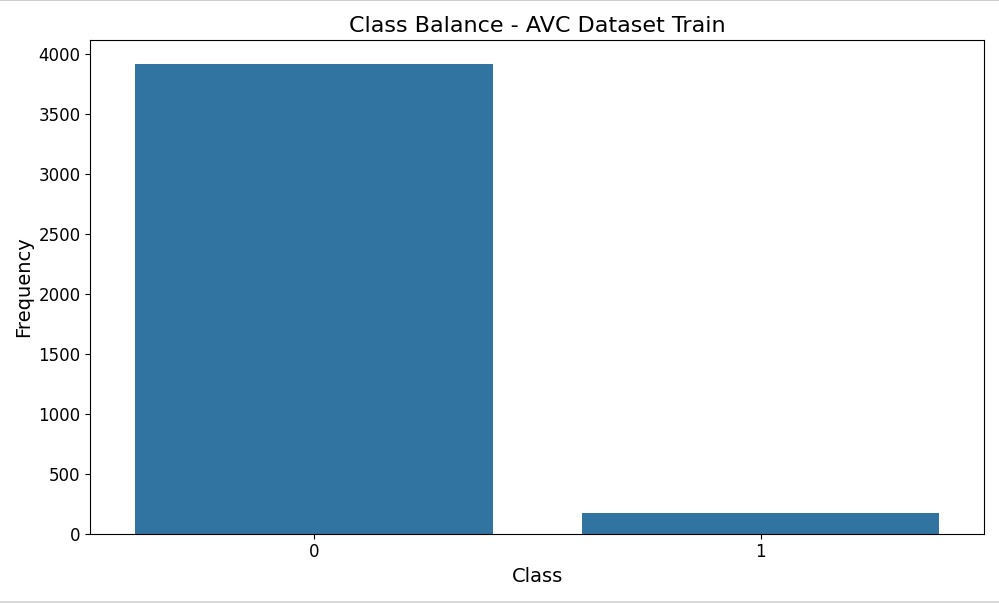
\includegraphics[width=0.8\textwidth]{Resources/class_balance_avc_train.jpeg}
    \caption{Class Balance - AVC Dataset Train}
\end{figure}


\newpage

\subsection{Salary Dataset}
\begin{figure}[h!]
    \centering
    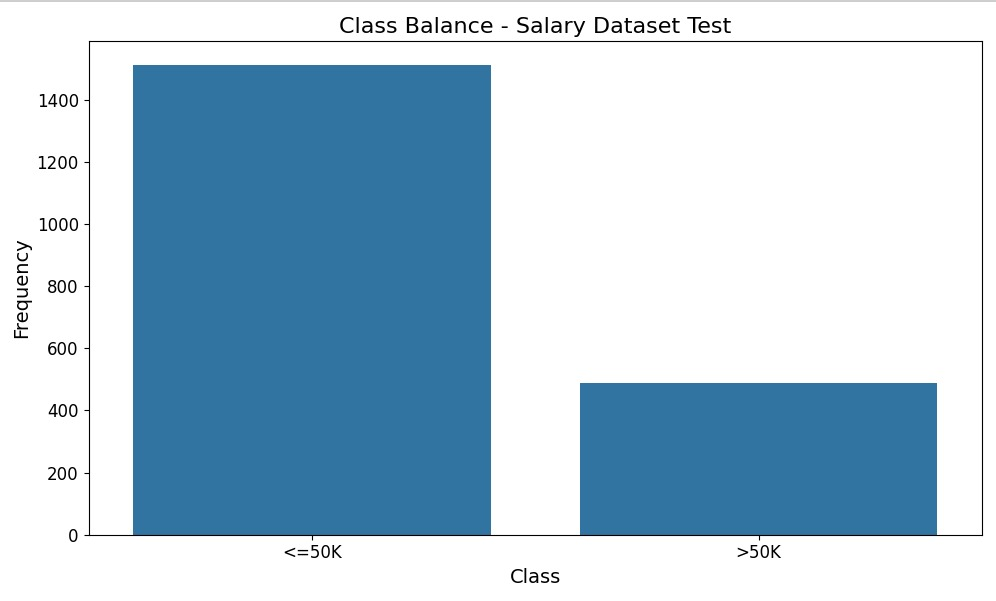
\includegraphics[width=0.8\textwidth]{Resources/class_balance_salary_test.jpeg}
    \caption{Class Balance - Salary Dataset Test}
\end{figure}

\begin{figure}[h!]
    \centering
    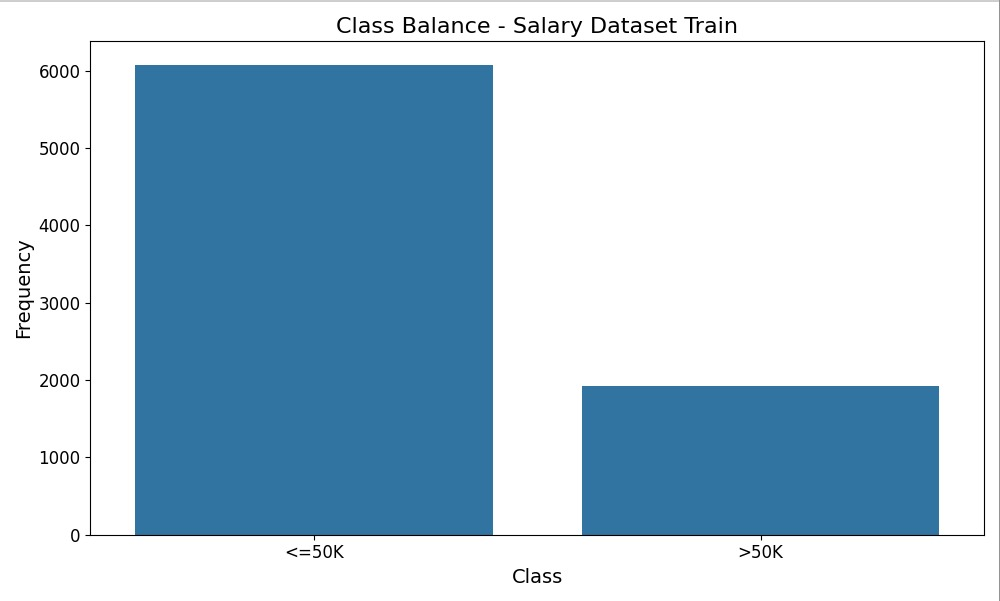
\includegraphics[width=0.8\textwidth]{Resources/class_balance_salary_train.jpeg}
    \caption{Class Balance - Salary Dataset Train}
\end{figure}

\subsection{Comments}
From the class balance plots above, it is evident that both datasets exhibit significant class imbalance. In the AVC dataset, the majority class (no stroke) is much more prevalent than the minority class (stroke). Similarly, in the Salary dataset, the class of individuals earning less than or equal to 50K is more common than the class of individuals earning more than 50K.

Class imbalance can have a substantial impact on model performance and evaluation. Models may become biased towards the majority class, leading to poor performance on the minority class. To address this, it is crucial to focus on evaluation metrics that provide a better understanding of performance on imbalanced datasets. Specifically, we should emphasize:

\begin{itemize}
    \item \textbf{F1 Score}: The harmonic mean of precision and recall, which provides a balance between the two.
    \item \textbf{Precision}: The ability of the classifier to not label a negative sample as positive.
    \item \textbf{Recall}: The ability of the classifier to find all positive samples.
\end{itemize}

By prioritizing these metrics, we can better assess and compare the performance of different algorithms on these imbalanced datasets.

\newpage
\section{Attribute Correlation}
This section presents the correlation matrices for both the AVC and Salary datasets. The correlation matrices are split into numerical and categorical attributes for both train and test sets.

\subsection{AVC Dataset}
\subsubsection{Numerical Attributes}
\begin{figure}[h!]
    \centering
    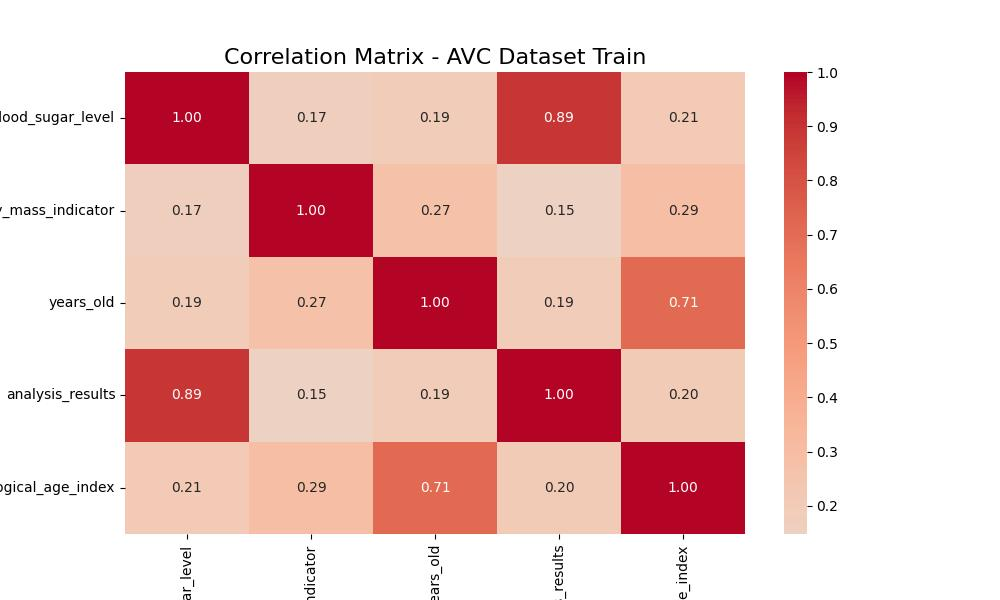
\includegraphics[width=0.8\textwidth]{Resources/matrix_avc_train.jpeg}
    \caption{Correlation Matrix - Numerical Attributes - AVC Dataset Train}
\end{figure}

\begin{figure}[h!]
    \centering
    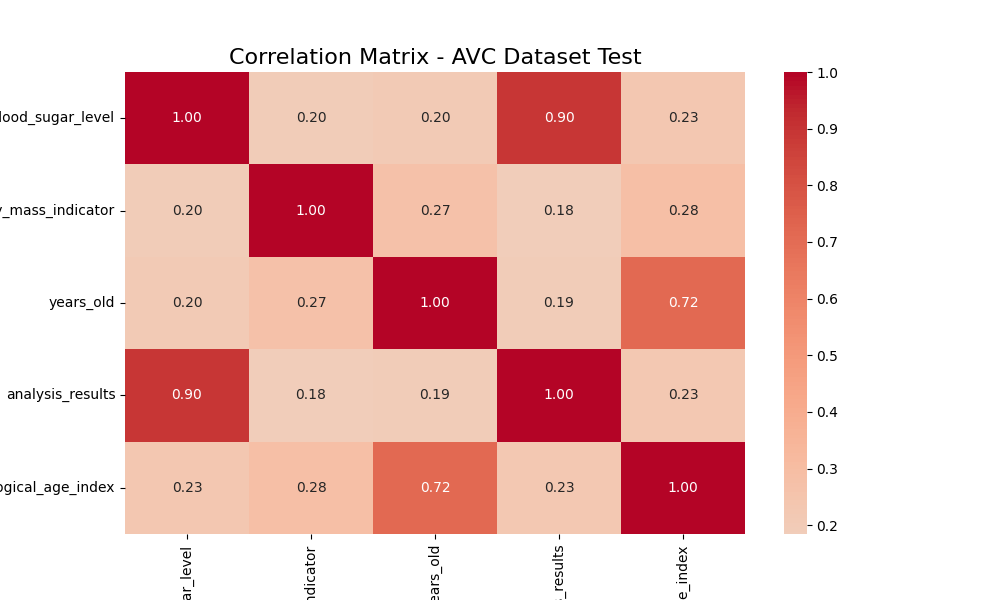
\includegraphics[width=0.8\textwidth]{Resources/matrix_avc_test.png}
    \caption{Correlation Matrix - Numerical Attributes - AVC Dataset Test}
\end{figure}

\newpage
\subsubsection{Categorical Attributes}
\begin{figure}[h!]
    \centering
    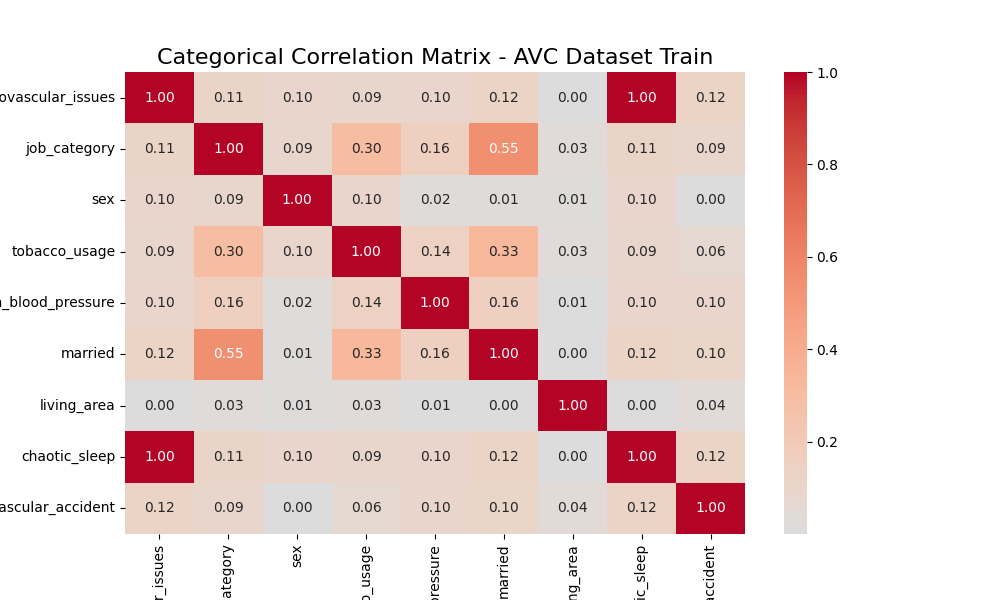
\includegraphics[width=0.8\textwidth]{Resources/matrix_categorial_avc_train.png}
    \caption{Categorical Correlation Matrix - AVC Dataset Train}
\end{figure}

\begin{figure}[h!]
    \centering
    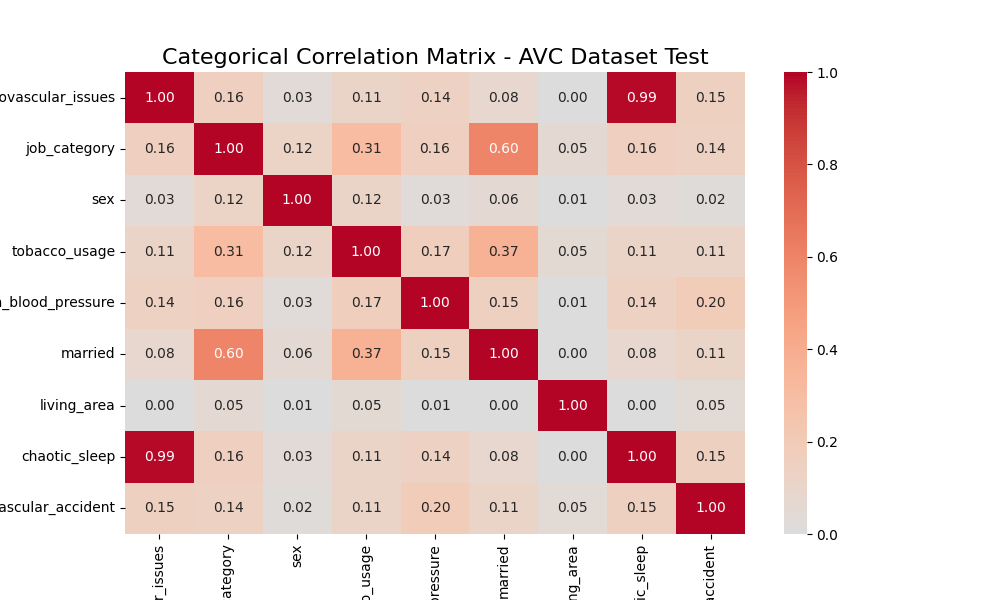
\includegraphics[width=0.8\textwidth]{Resources/matrix_categorial_avc_test.png}
    \caption{Categorical Correlation Matrix - AVC Dataset Test}
\end{figure}

\newpage
\subsection{Salary Dataset}
\subsubsection{Numerical Attributes}
\begin{figure}[h!]
    \centering
    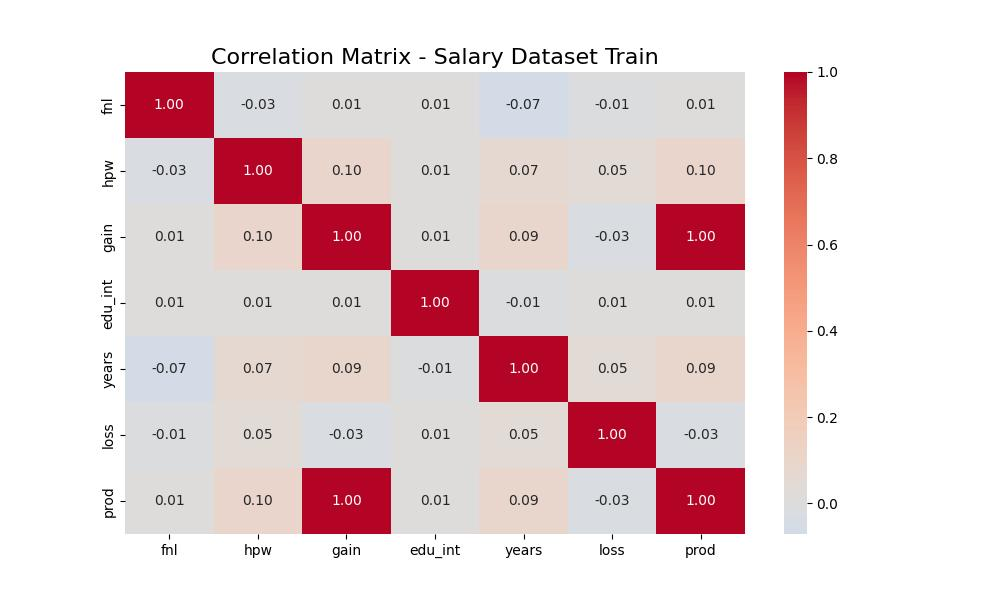
\includegraphics[width=0.8\textwidth]{Resources/matrix_salary_train.jpeg}
    \caption{Correlation Matrix - Numerical Attributes - Salary Dataset Train}
\end{figure}

\begin{figure}[h!]
    \centering
    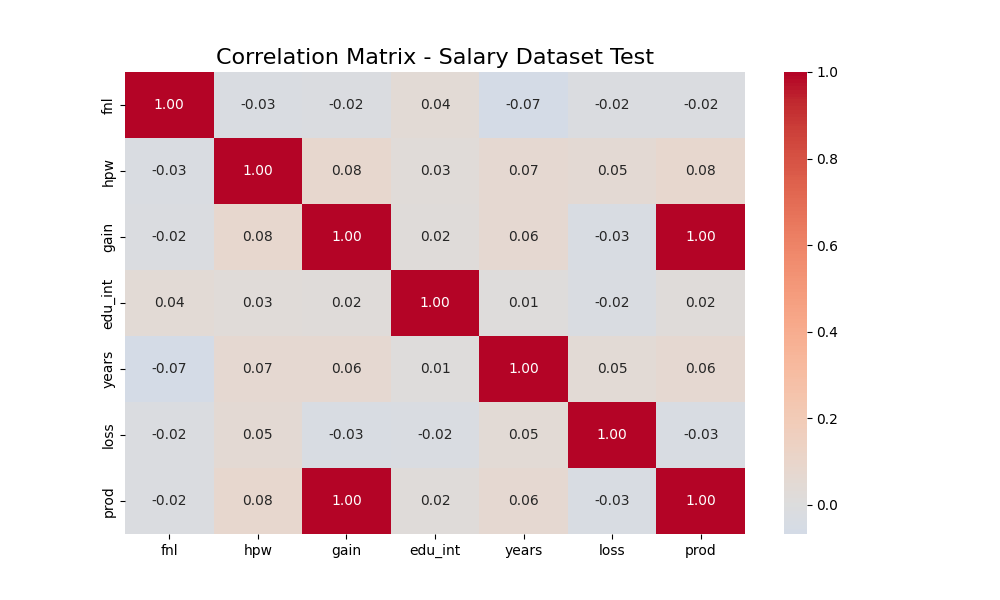
\includegraphics[width=0.8\textwidth]{Resources/matrix_salary_test.png}
    \caption{Correlation Matrix - Numerical Attributes - Salary Dataset Test}
\end{figure}

\newpage
\subsubsection{Categorical Attributes}
\begin{figure}[h!]
    \centering
    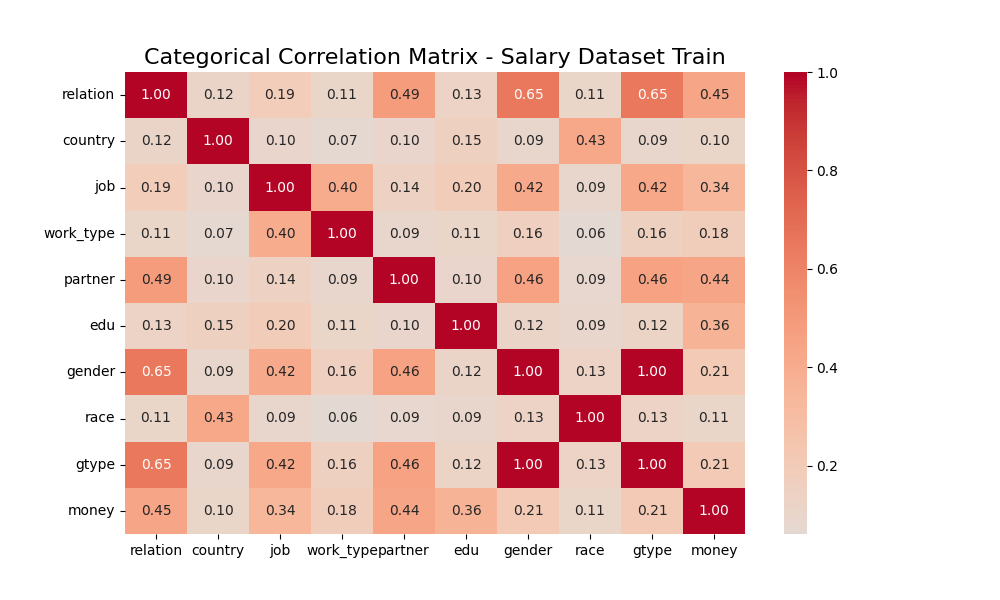
\includegraphics[width=0.8\textwidth]{Resources/matrix_categorial_salary_train.png}
    \caption{Categorical Correlation Matrix - Salary Dataset Train}
\end{figure}

\begin{figure}[h!]
    \centering
    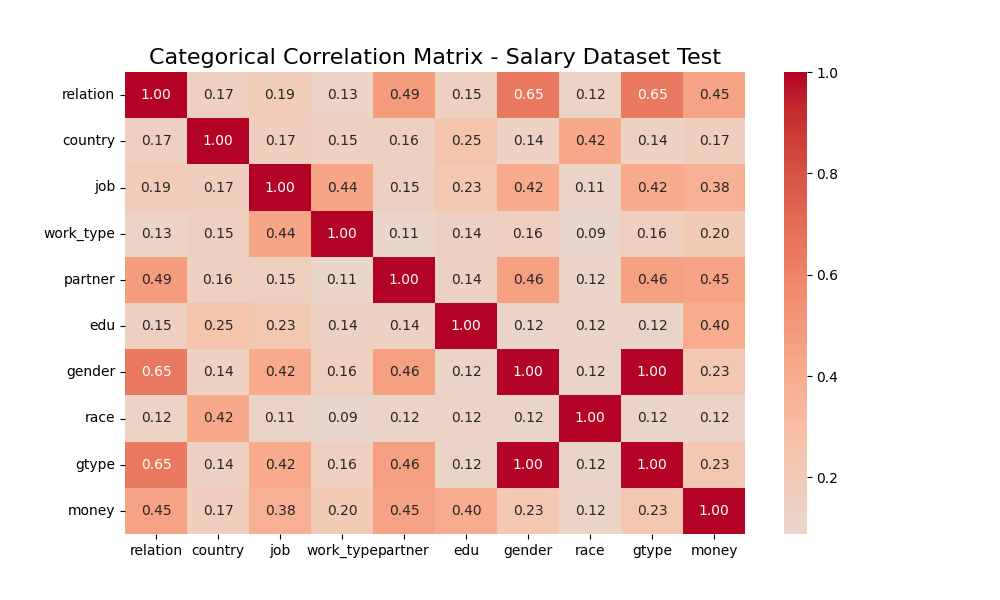
\includegraphics[width=0.8\textwidth]{Resources/matrix_categorial_salary_test.png}
    \caption{Categorical Correlation Matrix - Salary Dataset Test}
\end{figure}

\newpage
\subsection{Comments}
The correlation matrices provide insights into the relationships between different attributes in the datasets.

\subsubsection{AVC Dataset}
\paragraph{Numerical Attributes}
From the numerical attribute correlation matrices of the AVC dataset, it is observed that:
\begin{itemize}
    \item There is a moderate positive correlation between \textit{years\_old} and \textit{biological\_age\_index} in both train and test sets, which indicates that as the age of the person increases, the biological age index also tends to be higher.
    \item \textit{Analysis\_results} show a high correlation with \textit{blood\_sugar\_level}, but low with other numerical attributes, suggesting that the results of medical analyses are relatively independent of the person's age and other indicators.
\end{itemize}

\paragraph{Categorical Attributes}
The categorical correlation matrices for the AVC dataset indicate:
\begin{itemize}
    \item There are some moderate correlations between categorical variables such as \textit{married} and \textit{job\_category}, and \textit{job\_category} and \textit{tobacco\_usage}.
    \item These correlations suggest that there might be certain patterns or dependencies between the demographic and lifestyle attributes.
    \item There is a high correlation between \textit{chaotic\_sleep} and \textit{high\_blood\_pressure}, indicating that individuals with irregular sleep schedules are more likely to have high blood pressure.
\end{itemize}

\subsubsection{Salary Dataset}
\paragraph{Numerical Attributes}
For the Salary dataset, the numerical attribute correlation matrices reveal:
\begin{itemize}
    \item A strong positive correlation between \textit{gain} and \textit{prod}, indicating that individuals who gain more also tend to have higher produce of capital.
    \item \textit{Hours per week (hpw)} shows a low correlation with most other numerical attributes, suggesting that the number of hours worked per week is not strongly related to other numerical factors like capital gains or losses.
\end{itemize}

\paragraph{Categorical Attributes}
In the categorical correlation matrices for the Salary dataset:
\begin{itemize}
    \item Moderate correlations are observed between \textit{work\_type} and \textit{job}, as well as between \textit{country} and \textit{race}.
    \item These correlations highlight possible demographic and professional patterns.
    \item There is also a high correlation between \textit{gtype} and \textit{gender}, indicating that the type of work contract is directly influenced by the gender.
\end{itemize}

Overall, these correlation matrices help in understanding the interdependencies between attributes, which can be useful in feature selection and in improving the performance of machine learning models.

Eliminating specific variables such as \textit{analysis\_results} and \textit{biological\_age\_index} from the AVC dataset, and prod from the Salary dataset, can enhance the efficiency and performance of our machine learning models. These variables were identified as candidates for elimination due to their high correlation with other attributes, which makes them redundant, and their minimal impact on predictive accuracy. By removing these redundant or less impactful features, we reduce noise, prevent overfitting, and simplify the model, leading to improved generalization and more robust predictive performance. This streamlined approach allows the model to focus on the most significant attributes, enhancing both computational efficiency and model interpretability.
\end{document}
